\documentclass[11pt,a4paper]{article}

% Typeface: XeLaTeX with Latin Modern Roman (fontspec default)
\usepackage{fontspec}
\usepackage{polyglossia}
\setdefaultlanguage[variant=british]{english}

% Page: the measures of the note template (A4, 11 pt, 4.5 cm side margins, header and page count)
\usepackage[a4paper,left=4.5cm,right=4.5cm,top=4.5cm,bottom=4.1cm,headheight=14pt,headsep=0.55cm,
  footskip=0.55cm]{geometry}
\linespread{0.946}
\usepackage{fancyhdr}
\usepackage{lastpage}
\pagestyle{fancy}
\fancyhf{}
\fancyhead[L]{\small\textbf{PROJECT NOTE} $|$ Naive-Summation}
\fancyhead[R]{\small\textbf{Compiled on:} \notedate}
\fancyfoot[C]{\small\thepage\,/\,\pageref{LastPage}}
\renewcommand{\headrulewidth}{0.4pt}

\usepackage{microtype}
\usepackage{amsmath,amssymb}
\usepackage{booktabs,array,tabularx}
\usepackage{graphicx}
\usepackage{enumitem}
\setlist{noitemsep, topsep=3pt, leftmargin=*}
\usepackage{xcolor}
\definecolor{secblue}{HTML}{1F3A5F}
\definecolor{boxback}{HTML}{EEF2F6}
\definecolor{mark}{HTML}{9B2226}
\definecolor{hl}{HTML}{FFF36B}
\usepackage{titlesec}
\titleformat{\section}{\color{secblue}\bfseries\normalsize}{\thesection.}{0.4em}{}
\titlespacing*{\section}{0pt}{10pt}{4pt}
\usepackage[font=small,labelfont=bf,labelsep=period,skip=4pt]{caption}
\usepackage[bottom]{footmisc}

\setlength{\parindent}{0pt}
\setlength{\parskip}{5pt}
\setlength{\textfloatsep}{10pt}
\emergencystretch=3em

\newcommand{\notedate}{\number\day\space\ifcase\month\or January\or February\or March\or April\or May\or June\or
  July\or August\or September\or October\or November\or December\fi\space\number\year}

\newcommand{\SlopeNaivePos}{0.50}
\newcommand{\NormNaivePos}{237}
\newcommand{\NormPairPos}{0.55}
\newcommand{\NormKahanPos}{0.32}
\newcommand{\SlopeNaiveSym}{0.06}
\newcommand{\NormNaiveSym}{0.42}
\newcommand{\NormPairSym}{0.0025}
\newcommand{\NormKahanSym}{0.0005}
\newcommand{\CondTrials}{2,000}
\newcommand{\KappaMedian}{125}
\newcommand{\KappaMax}{181,407}
\newcommand{\CondSlope}{0.64}
\newcommand{\RelMean}{7.6\times 10^{-15}}
\newcommand{\RelMedian}{2.7\times 10^{-15}}
\newcommand{\MeanOverMedian}{2.8}
\newcommand{\TopShare}{37}
\newcommand{\KahanMaxEps}{1.00}
\newcommand{\BoundViolations}{0}
\newcommand{\TimeLoop}{17.9}
\newcommand{\TimeFsum}{15.1}
\newcommand{\TimeNpSum}{0.13}
\newcommand{\TimeKahan}{67}
\newcommand{\LoopOverFsum}{1.2}
\newcommand{\RefRatioPct}{0.54}
\newcommand{\Machine}{Darwin arm64, Python 3.13.6, NumPy 2.4.1}
\newcommand{\LongdoubleSentence}{On this machine \texttt{longdouble} has the same precision as \texttt{float64}, so the version 1 reference is simply NumPy's pairwise sum in double precision; its error is 0.5\% of the error of naive summation}


\begin{document}


\vspace*{14pt}
\begin{tabular}{@{}p{2.35cm}@{}p{\dimexpr\textwidth-2.35cm}@{}}
\textbf{TITLE:} & \textbf{\large Accuracy of naive summation: error growth, conditioning and better algorithms}\\[3pt]
\textbf{SUBJECT:} & Aim, method and results of the analyses in version 2 of the \texttt{Naive-Summation} repository\\[3pt]
\textbf{AUTHOR:} & Muhammed İkbal Yılmaz (myucanlar@gmail.com)
\end{tabular}

\vspace{8pt}
\vspace{12pt}

\section{Aim and scope}

Naive (recursive) summation computes $S = \sum_{i=1}^{n} x_i$ as $s_0 = 0$, $s_k = s_{k-1} + x_k$. In floating-point
arithmetic every addition is rounded, $\mathrm{fl}(a+b) = (a+b)(1+\delta)$ with $|\delta| \le \varepsilon$, where
$\varepsilon = 2^{-53} \approx 1.1\times10^{-16}$ is the unit roundoff of double precision. The computed sum
$\hat S$ therefore has an error $E = \hat S - S$. Version 1 of this project measured $E$ for random data and concluded that
naive summation is ``numerically unstable and unreliable''. This note asks three narrower questions, each answered by one
analysis:

\begin{enumerate}
  \item \textbf{How does the error grow with $n$,} compared with the theoretical bound, and does that depend on the data?
  \item \textbf{What makes the relative error $|E|/|S|$ large?} Version 1 found that it ``fluctuates''.
  \item \textbf{What do better algorithms gain, and at what cost?} And how accurate was the reference sum of version 1?
\end{enumerate}

\section{Method}

\begin{itemize}
  \item \textbf{Exact errors.} Every error is computed exactly: $\hat S$ and $-x_1, \dots, -x_n$ are added with
  \texttt{math.fsum}, which tracks the sum without intermediate rounding, and the result is rounded once. Comparing with a
  rounded reference sum instead would add up to half a unit in the last place to every error, which is as large as the
  error of the best algorithms. The unit tests check this against exact rational arithmetic.
  \item \textbf{Algorithms.} Naive summation (computed with \texttt{np.cumsum}, which the tests show is bit-for-bit the
  same as a Python loop and gives all partial sums at once); pairwise summation, which adds neighbours level by level;
  and Kahan's (1965) compensated summation, which carries the low-order part lost in each addition into the next.
  \item \textbf{Bounds} (Higham, 2002, ch.~4), with $\gamma_k = k\varepsilon/(1-k\varepsilon)$:
  naive $|E| \le \gamma_{n-1}\sum|x_i|$; pairwise $|E| \le \gamma_{\lceil \log_2 n\rceil}\sum|x_i|$; Kahan
  $|E| \le (2\varepsilon + O(n\varepsilon^2))\sum|x_i|$. Every error measured in the unit tests stays within these bounds.
  \item \textbf{Data.} Uniform random numbers as in version 1, $\mathrm{U}(-1,1)$, and for comparison $\mathrm{U}(0,1)$, where
  all terms have the same sign. Seeds are fixed.
\end{itemize}

\section{Analysis 1: Error growth (Figure~\ref{fig:growth})}

\textbf{Why.} The bound for naive summation grows linearly in $n$, and version 1 described the error as growing linearly.
But a bound is a worst case: it assumes that every rounding error has the largest size and the same sign. The question is
how the error grows in practice.

\textbf{Method.} For each distribution, 30 arrays of $10^6$ values; for 26 lengths $n$ between 10 and $10^6$ the error on the
first $n$ values is computed exactly. The figure shows the root mean square (RMS) of $|E|/(\varepsilon\sum|x_i|)$; in these
units the naive bound is the line $n-1$.

\textbf{How to read the figure.} Both axes are logarithmic, so a quantity that grows like $n^k$ appears as a line of slope
$k$. The distance between a curve and the dashed line shows how pessimistic the bound is.

\begin{figure}[h]
\centering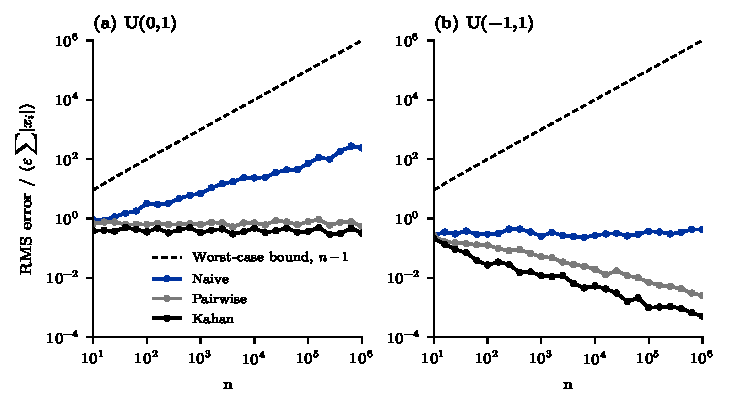
\includegraphics[width=\textwidth]{../figures/fig1_error_growth.pdf}
\caption{RMS error of three algorithms over 30 arrays, in units of $\varepsilon\sum|x_i|$. Dashed: worst-case bound for
naive summation.}\label{fig:growth}
\end{figure}

\textbf{Finding.} With positive terms, $\mathrm{U}(0,1)$, the naive error grows with slope \SlopeNaivePos{} on this scale:
like $\sqrt{n}$, as predicted when rounding errors behave like independent random signs (Johnson, 2019). At $n = 10^6$ it is
\NormNaivePos{} units, against $10^6$ for the bound. With terms of both signs, $\mathrm{U}(-1,1)$, the slope is only
\SlopeNaiveSym{}: the partial sums stay small, so each rounding error is small, and the error stays below one unit
(\NormNaiveSym{} at $n = 10^6$). In both cases pairwise and Kahan summation stay below one unit at every $n$ (at $n=10^6$:
\NormPairPos{} and \NormKahanPos{} for $\mathrm{U}(0,1)$; \NormPairSym{} and \NormKahanSym{} for $\mathrm{U}(-1,1)$).

\textbf{Interpretation.} ``The error grows linearly'' describes the bound, not the typical behaviour. How fast the error
actually grows depends on the data, through the size of the partial sums.

\section{Analysis 2: Conditioning (Figure~\ref{fig:cond})}

\textbf{Why.} The relative error of version 1 varied strongly from run to run. Dividing the naive bound by $|S|$ gives
$|E|/|S| \le \gamma_{n-1}\,\kappa$ with $\kappa = \sum|x_i|/|\sum x_i|$, the condition number of the sum. When terms of both
signs nearly cancel, $|S|$ is small and $\kappa$ is large, so even a small absolute error is a large relative error. This
analysis checks whether $\kappa$ explains the variation.

\textbf{Method.} \CondTrials{} arrays of $n = 10^4$ values from $\mathrm{U}(-1,1)$; for each, $\kappa$ and the exact relative
error of naive and Kahan summation.

\textbf{How to read the figure.} Each point is one array. Points that rise to the right mean that the relative error follows
the condition number.

\begin{figure}[h]
\centering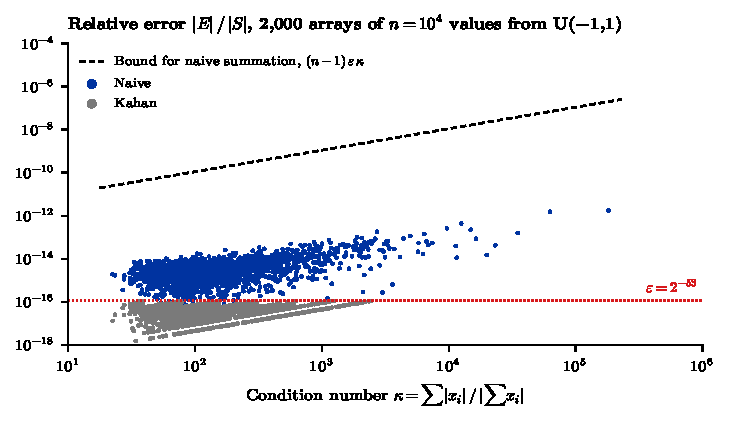
\includegraphics[width=\textwidth]{../figures/fig2_conditioning.pdf}
\caption{Relative error against the condition number for \CondTrials{} arrays of $10^4$ values from $\mathrm{U}(-1,1)$.
Dashed: bound for naive summation. Dotted: $\varepsilon$.}\label{fig:cond}
\end{figure}

\textbf{Finding.} The median $\kappa$ is \KappaMedian{}, the largest \KappaMax{}. The naive relative error rises with
$\kappa$ (slope \CondSlope{} on the log--log scale) and stays far below the bound (\BoundViolations{} violations). Its mean,
$\RelMean$, is \MeanOverMedian{} times its median, $\RelMedian$, because the 1\% of arrays with the largest errors account for
\TopShare\% of the mean: an average of relative errors, as in version 1, is dominated by a few sums close to zero. Kahan's
relative error never exceeds \KahanMaxEps{}$\,\varepsilon$, whatever $\kappa$; its points form bands because the result is
within one rounding of the exact sum, and roundings come in discrete steps.

\textbf{Interpretation.} The ``fluctuation'' is not instability of the algorithm but the conditioning of the problem.
Naive summation is backward stable: $\hat S$ is the exact sum of inputs perturbed by at most $\gamma_{n-1}$ in relative
terms (Higham, 2002, ch.~4; Johnson, 2019). A large relative error in an ill-conditioned sum is what any backward stable
method can produce.

\section{Analysis 3: Algorithms and the version 1 reference (Table~\ref{tab:algos})}

\textbf{Why.} A more accurate algorithm is only worth using if its cost is acceptable, so accuracy and time are measured
together. Version 1 used \texttt{np.sum(x, dtype=np.longdouble)} as the exact sum; the precision of \texttt{longdouble}
varies across platforms (NumPy documentation), so its accuracy is measured as well.

\textbf{Method.} 10 arrays of $10^6$ values from $\mathrm{U}(-1,1)$, as in version 1. Errors as in analysis 1; time is the
median of five calls (\Machine).

\begin{table}[h]
\centering\footnotesize
\caption{RMS error in units of $\varepsilon\sum|x_i|$ and running time for $n = 10^6$.}\label{tab:algos}
\begin{tabular}{lrr}
\toprule
Method & RMS error & Time (ms) \\
\midrule
Naive, Python loop (version 1) & 0.442 & 17.86 \\
Naive, \texttt{np.cumsum} & 0.442 & 2.09 \\
Pairwise & $1.9\times 10^{-3}$ & 0.47 \\
\texttt{np.sum} (NumPy, partial pairwise) & $2.4\times 10^{-3}$ & 0.13 \\
Kahan, Python loop & $4.2\times 10^{-4}$ & 67.10 \\
\texttt{math.fsum} (correctly rounded) & $4.2\times 10^{-4}$ & 15.13 \\
\texttt{np.sum}, \texttt{longdouble} (version 1 reference) & $2.4\times 10^{-3}$ & 0.13 \\
\bottomrule

\end{tabular}
\end{table}

\textbf{Finding.} The Python loop of version 1 is both inaccurate and slow: it takes \TimeLoop{} ms,
while \texttt{math.fsum}, whose result is the exact sum correctly rounded, takes \TimeFsum{} ms (\LoopOverFsum{} times
faster) and \texttt{np.sum} takes \TimeNpSum{} ms with an error two orders of magnitude smaller. Kahan's method reaches the
accuracy of \texttt{fsum} but is slow when written in Python (\TimeKahan{} ms); its advantage is that it needs only a constant
amount of extra work per term, which matters in compiled code. \LongdoubleSentence. Measuring errors against an exact
reference, as done here, avoids this platform dependence.

\section{Conclusions and limitations}

\begin{itemize}
  \item The error of naive summation is far below its worst-case bound. It grows like $\sqrt{n}$ on the bound's scale for
  terms of one sign and hardly grows for terms that cancel. The relative error is governed by the condition number.
  \item Naive summation is backward stable, not unstable. For accurate sums in Python, \texttt{math.fsum} is both correctly
  rounded and faster than a Python loop; \texttt{np.sum} is fast and much more accurate than naive summation.
  \item Only uniform data, double precision and sizes up to $10^6$ were studied. Times were measured on a single machine.
\end{itemize}

\section*{References}
{\small
\setlength{\parskip}{2pt}
\hangindent=1.27cm\hangafter=1 Higham, N. J. (1993). The accuracy of floating point summation. \textit{SIAM Journal on Scientific Computing}, 14(4), 783--799.\par
\hangindent=1.27cm\hangafter=1 Higham, N. J. (2002). \textit{Accuracy and Stability of Numerical Algorithms} (2nd ed.). SIAM.\par
\hangindent=1.27cm\hangafter=1 Johnson, S. G. (2019). Notes on the accuracy of naive summation; and Backwards stability of recursive summation.
MIT course 18.335J, \textit{Introduction to Numerical Methods}, Lecture 3.\par
\hangindent=1.27cm\hangafter=1 Kahan, W. (1965). Further remarks on reducing truncation errors. \textit{Communications of the ACM}, 8(1), 40.\par
\hangindent=1.27cm\hangafter=1 NumPy documentation: \texttt{numpy.sum}, \texttt{numpy.cumsum}, \texttt{numpy.finfo}. Python documentation: \texttt{math.fsum}.\par

\smallskip
All numbers are generated from
\texttt{figures/*.csv} by \texttt{make\_paper.py}.
}

\end{document}
